\section{Requirements Engineering for BX}
\label{section:requirements}

In this section we will consider techniques and tools for requirements engineering for BX. We will motivate the benefits of considering requirements for BX in general, before discussing some of the general questions to be addressed when building a BX. These questions will help us motivate a discussion on the general properties of BX (which may be the source of constraints on requirements for a BX), as well as examples of functional and non-functional requirements for BX. This is followed by a broad overview of requirements engineering processes for BX, which leads in to a discussion on requirements specification languages suitable for BX.

\subsection{Motivation}
Requirements engineering is the process of identifying, documenting and maintaining requirements in systems engineering. The typical tasks involved in requirements engineering are:
\begin{itemize}
\item \textit{identification:} where new requirements to address a problem are clarified
\item \textit{analysis:} where the requirements are assessed to ensure they accurately capture what is needed for the system under consideration, and conflicts between stakeholders are resolved
\item \textit{specification:} where the requirements are documented in a precise (but not necessarily formal) way
\item \textit{validation:} where the requirements are checked to ensure they are consistent and address stakeholder needs
\item \textit{maintenance:} where the requirements are considered for update as the system under consideration is constructed, deployed and changed.
\end{itemize}
BX are software systems and as such will benefit from a clear understanding of requirements; for large or complicated BX, there may be benefits to following a rigorous requirements engineering process as well. In particular, an understanding of requirements for BX can help in mapping BX problems to tools that are suitable for implementation (and vice versa). An understanding of requirements for BX can also help in contrasting different potential solutions in terms of their tradeoffs in how they satisfy requirements.  

\subsection{Questions and Properties for BX}
A typical first phase of requirements engineering is \textit{identification}, where engineers attempt to determine what requirements a software system should exhibit. This in turn may help determine properties or constraints that the ultimate system will satisfy. There are numerous ways in which requirements can be identified, e.g., via stakeholder interview, by reviewing existing similar systems, by following questionnaires or checklists, or by using testing techniques to derive requirements. Based on \cite{TehraniZL16} we suggest some general questions that could be addressed when constructing a BX, the answers to which could help derive requirements.

\begin{enumerate}
\item What needs to be transformed into what?
\item What mechanisms can be used for building the BX? (i.e., theory, tools, techniques)
\item What are the application domains for the BX?
\item What are the specific characteristics of the BX (e.g, what patterns are appropriate to use)?
\item What are the quality requirements (e.g., performance) for the BX?
\item What are the success criteria for the BX?
\end{enumerate}
Questions 3, 4 and 6 are possibly the most opaque. Question 3 is designed to help identify constraints on the scope of use for the BX, e.g., will the BX be used in developing hard real-time systems, or interactive systems? Question 4 is designed to help identify functional requirements, e.g., should the BX be parameterised, should it be interactive? This in turn may help identify suitable patterns that can be used in specifying or designing the BX. Question 6 is the ``stopping condition'': how will we know if we have successfully solved the BX problem?

BX exhibit various properties (such as least-change, or determinism). When considering requirements for a BX, there are general properties that may be of interest, particularly in determining constraints that the ultimate BX must satisfy. Some examples are:
\begin{itemize}
\item Size: is the BX small (e.g., a single reversible refactoring) or large (e.g., a reversible code generator)? 
\item Level of automation: is the BX meant to be fully automated, or involve a human-in-the-loop?
\item Visualisation: how is the BX, its results, and its input presented to users?
\item Level of industry application: to what extent is the BX to be deployed in an industrial context?
\item Maturity level: should the BX be implemented in a tool? Should the BX be a theoretical construct?
\end{itemize}
Understanding the relative importance of these properties will be helpful in deciding on what theory or tool to choose for defining a BX.

\subsection{Functional and Non-functional Requirements}
In the classical requirements engineering literature, functional requirements specify what a system must, could or should provide. Non-functional (or behavioural) requirements specify criteria against which we can judge the quality of a system. In a requirements document, functional and non-functional requirements are typically presented separately, with suitable tests given that can be used to assess the coverage and completeness of fulfilment of requirements.

There has been little published research on examples of requirements for transformations in general, let alone BX, but based on \cite{TehraniZL16,NalchigarSC13} we can propose some examples for BX. We start with functional requirements. For simplicity of presentation, we assume that a BX under development is defined between two models (a source and a target).

\begin{itemize}
\item \textit{Correctness:} when the BX is run in the forward direction, the target model must be well formed (defined in terms of conformance to the target metamodel and any corresponding constraints). Similarly, when the BX is run in the reverse direction, the source model must be well formed.

\item \textit{Inconsistency tolerance:} the BX should be able to support incomplete or inconsistent models, e.g., temporarily inconsistent models. This reflects the practical situation wherein a BX \textit{gradually} re-establishes consistency over a sequence of steps.

\item \textit{Modularity:} it should be possible to compose BX into new transformations.

\item \textit{Traceability:} a BX should support the generation of trace-links (sometimes called a correspondence model) between source and target models, as well as between the steps of a transformation chain.

\item \textit{Change propagation:} a BX should provide support for propagating changes from one model to the other model. 

\item \textit{Incrementality:} a BX should make it possible to update a model based only on the changes made to the other model (that is, the parts of the model that do not change are not used to make changes to the other model). 

\item \textit{Uniqueness:} a BX could support the ability to generate a unique solution to the problem of ensuring consistency between two models.

\item \textit{Termination:} it should be possible to support the definition of terminating BX transformation executions.

\item \textit{Style:} a BX should be expressible in a particular style, i.e., declarative, operational or hybrid. 
\end{itemize}
Note the wording of these requirements; we have used the words \textit{must}, \textit{should} and \textit{could} to indicate the degree of importance or criticality of each type of requirement. As this suggests -- and as is reinforced by \cite{HidakaTCH16} there is substantial variability in what BX provide (and also how they are implemented).

Non-functional requirements, recall, specify criteria against which we can judge the quality of a BX. As is the case for functional requirements for BX, there is limited research on non-functional requirements. Some examples have been proposed in \cite{NalchigarSC13}, and we list a selection here.

\begin{itemize}
\item Extensibility: the extent to which the BX can be extended to support new functional requirements  or a change in scope.

\item Usability: is the BX judged to be usable by stakeholders?

\item Robustness: can the BX manage invalid models (i.e., that do not conform to the metamodels involved in the BX), or deal with errors in models?

\item Interoperability: can the BX be combined and used together with non-BX tools (e.g., other MDE tools and operations, such as model comparisons or mergings)?
\end{itemize}

Clearly, more research on requirements for BX is needed. As our experience with building BX grows, and our understanding of what constitutes a useful BX scenario increases, our ability to elaborate sensible functional and non-functional requirements for BX will improve.

\subsection{Requirements Engineering Processes for BX}
In this section we briefly outline typical stages of a requirements engineering process for BX and highlight the key artefacts and stakeholders that will be involved. We also point out some of the problems that might arise during requirements engineering. This leads in to the next section where we give an overview of some of the key techniques that can be used within a requirements engineering process for BX.

The requirements engineering literature, e.g., \cite{ieee-29148-2011}, identifies the following generic phases in requirements engineering:
\begin{itemize}
\item \textit{Domain analysis and elicitation:} Identify who are your stakeholders. From these stakeholders, gather information on the system domain and system requirements.

\item \textit{Evaluation and negotiation:} Identify imprecision, conflicts, omissions and redundancies in the informal requirements identified in the previous phase.  Resolve these (if possible and appropriate) via negotiation and consultation.

\item \textit{Specification:} Document the formal requirements in a specification (we will consider this for BX in more detail later). The specification is often the basis for a contract between developers and customers.

\item \textit{Validation and Verification:} Check the specification for consistency, completeness and acceptability to stakeholders.
\end{itemize}

This is generic, applicable to any kind of software or systems engineering. What might a requirements engineering process for BX look like? Tehrani et al \cite{TehraniZL16} propose a process for transformations, which is depicted in Figure~\ref{fig:re-process}.

\begin{figure}[htbp]
\centering{\scalebox{0.6}{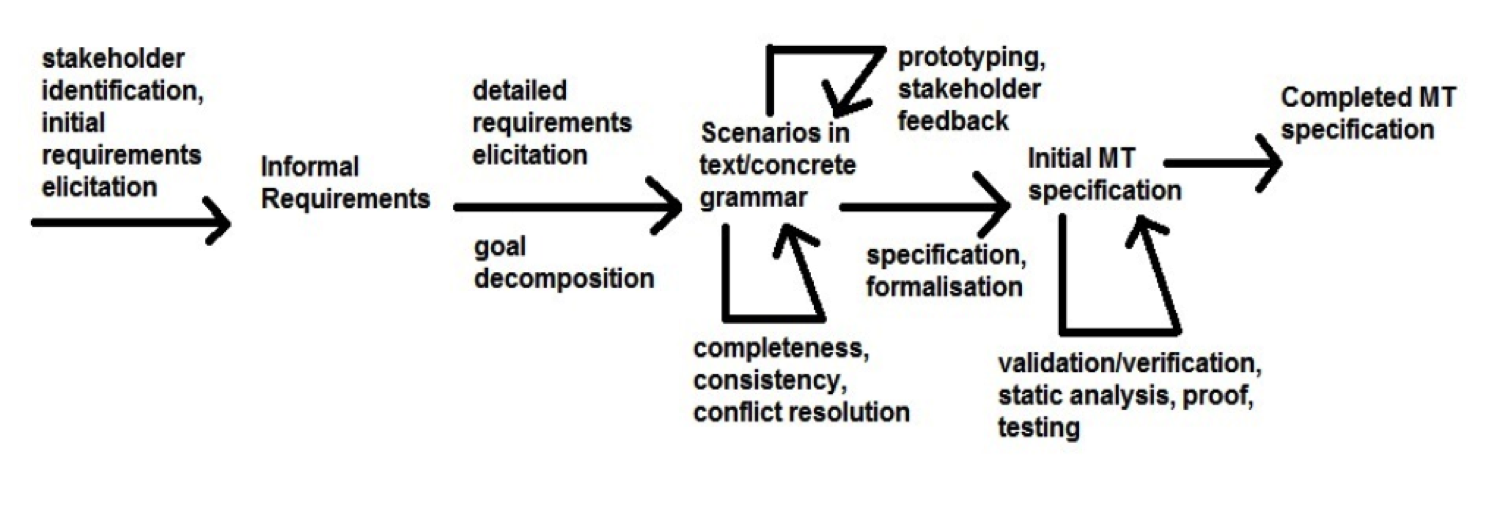
\includegraphics{re-process-bx.png}}}
\caption{A requirements engineering process from \cite{TehraniZL16}}
\label{fig:re-process}
\end{figure}
(It is worth emphasising that the process shown in Figure~\ref{fig:re-process} is for transformations in general, not specifically for BX.) There are some points to note about the above process.

\begin{itemize}
\item The process is generic for the most part, and resembles the steps that are typically carried out for software systems.

\item An interesting aspect is the use of scenarios as a concrete mechanism for driving the development of a requirements specification. In the context of BX this suggests that identifying and capturing more (and more detailed) BX scenarios will be very helpful in improving our understanding of BX requirements engineering.

\item The process distinguishes between local and global requirements, as is often done in systems engineering. A local requirement may pertain to a particular transformation component (e.g., that correspondences are defined between elements of particular types), whereas a global requirement may apply to an entire transformation (e.g., a performance requirement, that a measure of complexity is reduced by running a BX, or a safety requirement).
\end{itemize}

\subsection{Elicitation}
\textit{Elicitation} is an important first step in any requirements engineering process. What techniques might be applicable for BX? Many of the traditional elicitation techniques appear to be directly applicable to BX problems with little change, as argued by Tehrani et al \cite{TehraniZL16}. For example, a classic elicitation technique is observation (an ethnographic method): observing an existing -- possibly manual -- BX technique or process could provide sensible requirements for an automated process. Consider a scenario wherein a BX is to be defined between an Excel spreadsheet and a SysML requirements diagram\footnote{This is a sanitised version of a real problem encountered by the author.} A manual BX process between the two might involve (a) making changes to cells in an Excel column; (b) switching to a SysML editor; and (c) modifying attributes in a SysML class model. This might indicate to a requirements engineer a sequence of steps that is needed to implement in an automated BX.

Another technique that can be used for elicitation is the \textit{unstructured interview}, where open-ended questions are asked about the problem domain or the current (BX) process. This can be useful for identifying transformation goals, e.g., ``ensure that the source and target models are inconsistent for no more than 10ms''. In carrying out an unstructured interview regarding a transformation, Tehrani \cite{TehraniZL16} suggests some generic open-ended questions that may be useful to consider; we have extended their questions with some of our own, based on our experience in the MONDO project\footnote{http://www.mondo-project.org/}.
\begin{itemize}
\item Is there a size range for the source and target models? This may suggest to the engineer the type of infrastructure that may be useful for the project (e.g., EMF to represent models).

\item Does the encoding for the BX matter? For example, for very large scale models it may be necessary to consider binary formats.

\item Are there any assumptions that are made about the source or target models? For example, are they always available? Are they read-only? Write-only? Are there confidentiality restrictions?
\end{itemize}
Along with unstructured interviews there are \textit{structured} interviews, which involve asking pre-loaded questions about the domain and the BX, perhaps based around a checklist linked to a requirements pattern catalogue. For example, a checklist of questions may be divided into parts, one focusing on questions related to global functional requirements (e.g., is hippocraticness important, is semantics preservation important?) and another related to local non-functional requirements (e.g., should this rule satisfy a specific time bound?)

A final elicitation technique that we mention is \textit{scenario-based analysis}, where scenarios are used to capture different requirements transformation processing cases. The benefit of using scenarios is that they are concrete: scenarios are usually presented in a concrete scenario language, often supplemented with sketches of sample models. 

\subsection{Evaluation}



